\section{Introduction}

\subsection{Subsections appear like this}
\subsubsection{And  sub-subsections appear like this}

Equations are defined in the \{equation\} environment:
 \begin{equation}
\frac{n!}{k!(n-k)!} = \binom{n}{k}
\end{equation}

\begin{equation}
\lim_{x \to \infty} \exp(-x) = 0
\end{equation}

Citations may either be inline: \citet{einstein1935particle} or in parentheses \citep{einstein1935particle}.

The main body of the text should go here, with footnotes\footnote{such as this one} used when appropriate.
\section{Lipsum}
\lipsum

\begin{figure}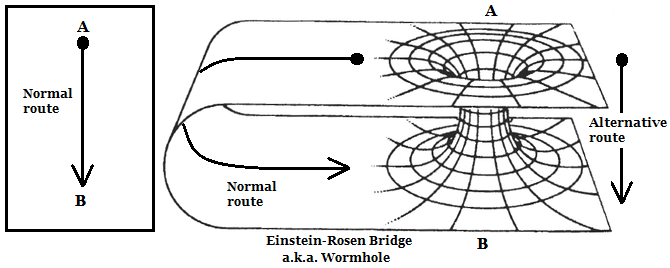
\includegraphics[width=\columnwidth]{ER-bridge}
\caption{Einstein--Rosen bridge (``wormhole'').}
\label{fig:1}
\end{figure}
\section{More Lipsum}

\lipsum
